\documentclass[reprint, aps, pra, nofootinbib, floatfix]{customrevtex}   % Implement custom class based on REVTeX

%%%%%%%%%%%%%%%%%%%%%%
% Change numbering to bottom center
\makeatletter
\def\ps@article{%
  \def\@oddfoot{\hfil\normalsize\thepage\hfil}  % Center page number at bottom
  \def\@evenfoot{\hfil\normalsize\thepage\hfil}  % Same for even pages
  \let\@oddhead\@empty  % Remove header from odd pages
  \let\@evenhead\@empty % Remove header from even pages
}
\pagestyle{article}
\makeatother
%%%%%%%%%%%%%%%%%%%%%%


%%%%%%%%%%%%%%%%%%%%%%
% Input packages and commands
% and set bibliography style
%%%%%%%%%%%%%%
% Page Style %
%%%%%%%%%%%%%%
\usepackage[margin=0.7in]{geometry}   % Setting margins
\usepackage{hyperref}               % Permit clickable web links
\usepackage{enumitem}               % Better enumerate environment
\usepackage{multirow, booktabs}     % Better tabular commands


%%%%%%%%
% Math %
%%%%%%%%
\usepackage{physics}                % Better math symbols common to physics
\usepackage{siunitx}                % Easy SI unit expressions
    \sisetup{separate-uncertainty=true} % Use plus-minus form of uncertainty
    \sisetup{per-mode = symbol}         % Use "/" instead of "^{-1}" for inverse units
\usepackage{mathtools}              % Beautify math and add some useful commands
\usepackage{bm}


%%%%%%%%%%%
% Figures %
%%%%%%%%%%%
\usepackage{graphicx}				% Including figure/image
\usepackage{wrapfig}                % Enable wrapping text around figures
%%%%%%%%%%%%%%%%%%%%%%%%%%%%%%%%%%%%%%%%%%%%
% Place new global commands here to replace
% long, reptitive math equations or text
%%%%%%%%%%%%%%%%%%%%%%%%%%%%%%%%%%%%%%%%%%%%
\bibliographystyle{apsrev4-2}
%%%%%%%%%%%%%%%%%%%%%%


%%%%%%%%%%%%%%%%%%%%%%
% Easy-change commands for affiliations
\newcommand{\projTitle}{Project 1}      % Title goes here
\newcommand{\name}{John Doe}            % Name goes here
\newcommand{\duedate}{---, 2025}        % Due date goes here
%%%%%%%%%%%%%%%%%%%%%%


\begin{document}

%%%%%%%%%%%%%%%%%%%%%%
% Title and affiliations
\title{\projTitle}
\author{\normalsize\name}
    \affiliation{\normalsize Department of Physics \& Astronomy\\University of Kentucky\\ \duedate}
%%%%%%%%%%%%%%%%%%%%%%


%%%%%%%%%%%%%%%%%%%%%%
% Abstract
\begin{abstract}
\normalsize
A research paper begins with a short abstract containing a summary of the aims, the methods, and the results of the investigation. Your paper’s abstract should therefore contain a clear statement of the overall nature of your project, and include a summary of how the work was done. You might write, for example: We have determined the elementary unit of electrical charge, e, by measuring the terminal speed of ten charged oil drops in a uniform electric field. An abstract should also contain your estimate of the true value of the measured quantity and its error – assuming you have only one or two such values to report. For example, you could write: We find the charge of the electron to be $\SI{-1.73(22)e-19}{\coulomb}$. Note that only 2 significant figures are given in the error, and the least significant digit (LSD) of the error corresponds to the LSD of the quoted mean value.
\end{abstract}
%%%%%%%%%%%%%%%%%%%%%%


\maketitle   % abstract is include in 'title', so \maketitle command is listed here


%%%%%%%%%%%%%%%%%%%%%%%%%%%%%%%%%%%%%%%%%%%%
% Commands to input sections of paper.
% DO NOT write content in this area, use
% the tex files in the 'section' folder

\section{Introduction} \label{sec:introduction}

The introductory section of your paper is intended to give the reader a clear picture of the scope and significance of your project. In most papers, the introduction includes a discussion of at least some of the previous relevant measurements, often commenting on their relative strengths and weaknesses. Since nearly all of the projects we will do have historical significance, the introduction to your report can briefly describe how the phenomena you are investigating have played a role in helping to define our present understanding of physics. And usually, an introductory section of a paper concludes with one or two sentences indicating the topics which are covered in each of the paper's subsequent sections. 

Most importantly, the introduction should present an overview of the entire project. A reader not familiar with the science will then be able to develop a broad picture of your work, before they delve into the more detailed discussion. By presenting the project's landscape early in the paper, the reader will be able to more readily comprehend the details of the project as they are subsequently offered.

You can use this file as the template of your paper. It is available for download from the Modules section of our Canvas page. The LaTeX word processing software used to create and edit this file is freely available for both PC and MAC machines at \href{https://www.overleaf.com}{Overleaf.com}. If you choose not to use Overleaf, then your word processing software should be set up to create a document with 12-point font for the main text and 0.7-inch margins on all sides. Your paper must be 5 or 6 pages in length, excluding the references and appendix.

\subsection{Important Considerations}

    As you prepare your paper, you should keep several other points in mind. Strive to achieve clarity and accuracy in your writing.

    Scientists work hard in a laboratory to make precise measurements, and they value a written report which avoids misrepresentations, ambiguities, and outright errors. 

    Imagine that your reader is another physics major not enrolled in this course. Your goal will be to produce a document which they can readily comprehend -- or, at least one which they can understand after a second reading. This can most easily be achieved by "telling the story" of your lab work. Like all stories, yours will include a beginning, a middle, and an ending. The introduction serves as the beginning of the story, followed by the development section, which provides a detailed account of your work and the final results. The ending of your story will include an interpretation of the measured data within the context you have previously established earlier in your paper.

    The first sentence of each paragraph should make a significant statement about one element of the project. The sentences which follow in each paragraph should amplify and clarify the information contained in the first. Someone should be able to read just the first sentence of each paragraph in the paper and glean a relatively thorough understanding of the project.
    
    Your written description of the methods used to obtain and analyze the data should be written in the past tense. Use the present tense when you write the conclusions. Note that your paper will be evaluated for its use of proper grammar and spelling. Please also note that in printed text the word "data" is treated as a plural noun. The singular form is "datum."
\section{Theory}\label{sec:theory}

In general, the single most important element of a research paper in our field is the physical insight which it conveys. In some cases, this is achieved by relating the results of our laboratory measurements to the predictions of an underlying theory. In other cases, our data provide information on one or more parameters which are elements of a physical theory. An example of the former is our study of the photoelectric effect, in which Einstein's very simple formula relating the work function, the frequency of light, and the maximum energy of the ejected electron is tested against measured data. Alternately, our experiment to measure the charge on the electron provides the value of e, which is not predicted by any theory.

The Theory section of your paper should provide a clear description of the physical phenomenon you are studying. It will typically include one or a few important mathematical results. For example, a paper on the photoelectric project will cite Einstein's result,\cite{Marg_88}
\begin{equation}\label{eq:photoelectric_energy}
    T_{\text{max}}=hf-\phi,
\end{equation}
where $T_{\text{max}}$ is the electron's maximum kinetic energy, $h$ is Planck's constant, $f$ is the frequency of the light, and $\phi$ is the work function. Notice first that each formula is separated from the text and sequentially numbered, and that each symbol appearing in the equation is defined in the text. Equation 1 could be used as the starting point for your description of the physical mechanism of the photoelectric effect.

Another example is provided by the oil drop experiment. In that case, equations are used to relate the measured rise and fall times of the drops to their charge. You should not derive these results, but instead they should simply be stated, with a citation, in the Theory section of your paper.

Overall, the content of this section will form the basis for your subsequent interpretation of your measured data.
\section{Experimental Methods} \label{sec:experiment}

In this section, you should provide a description of your experimental equipment, including enough detail for the reader to understand not only the physical layout but also the usage of the equipment.

\begin{figure}[ht]
    \centering
    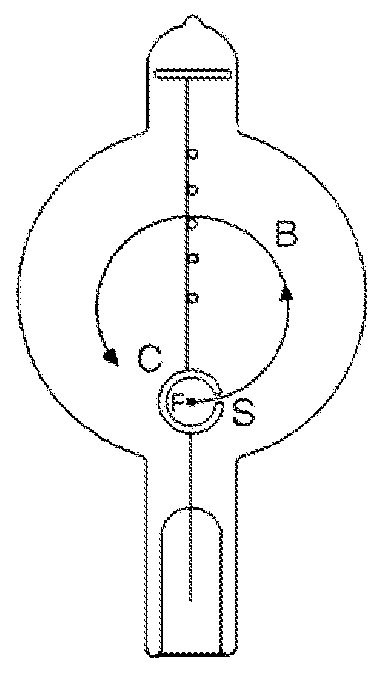
\includegraphics[width=0.4\linewidth]{figures/evacuated_tube.png}
    \caption{\footnotesize The evacuated tube used to measure the orbit radius of the electron beam in an external magnetic field. Electrons emitted by the filament (F) are collimated by a slit (S) and form a narrow beam (B). The crossbar (C) contains five markers at known orbit radii.}
    \label{fig:evacuated_tube}
\end{figure}

Present a figure showing the essential features of the apparatus early in this section, usually as a schematic drawing rather than a photograph. Refer to this figure within your text as Fig. 1; for example: A schematic representation of the apparatus used to measure the electron charge-to-mass ratio is shown in Fig. \ref{fig:evacuated_tube}. Then, locate this figure close to the text in which it is referenced. Notice that each figure contains a caption which provides a useful explanation of the figure's contents. Typically, figure and table captions use 10-point font.
\section{Results}\label{sec:results}

Having already described both the apparatus and the method by which your data were acquired, it is now time to present your results.

\begin{figure}[ht]
    \centering
    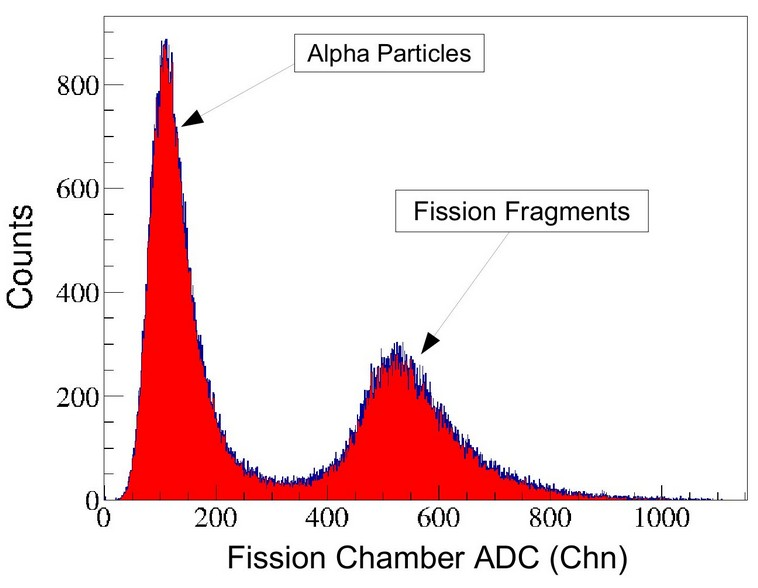
\includegraphics[width=0.8\linewidth]{figures/fission_spectrum.png}
    \caption{\footnotesize The measured energy spectrum in the fission chamber. The separate peaks are from alpha particles emitted in the radioactive decay of $\prescript{238}{}{\text{U}}$, and nuclear fragments created by neutron-induced fission.\cite{Kov_22}}
    \label{fig:fission_spectrum}
\end{figure}

In many experiments, the 'raw data' consist of a measured spectrum of one form or another. In such a case, you should present just one example spectrum, such as the one shown in Fig. \ref{fig:fission_spectrum}. Either on this figure, or in its caption, make note of any important spectral features. The text of your paper should expand on the short description contained in the figure caption.

In other types of experiments, the data consist of a set of measured x-y values. You might have used, for example, a digital voltmeter (DVM) to measure the photocurrent produced by the photoelectric effect when you illuminated a metal surface with a steady light source. The dependent variable is the measured current, while the independent variable is the applied retarding potential. Your measurements would then consist of a number of x-y data points, and these should be shown in your paper. (You may actually have collected several such data sets, but only one set should appear as a figure in the paper. You should, however, mention these additional data in the text.) We show in Fig. \ref{fig:photocurrent} an example plot of a complete x-y data set.

\begin{figure}[ht]
    \centering
    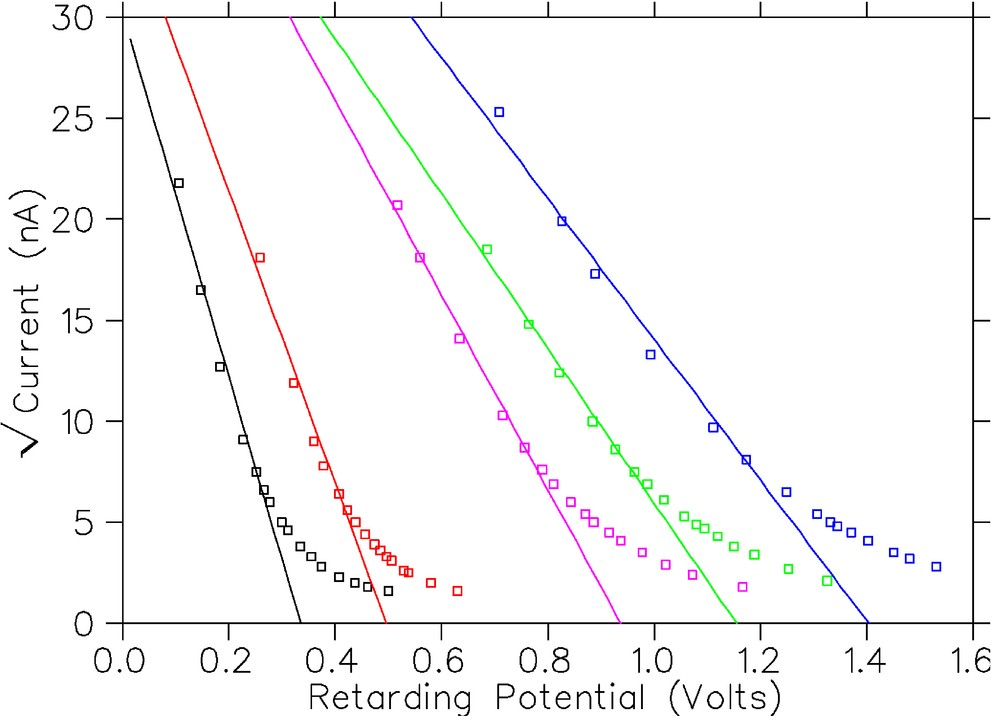
\includegraphics[width=0.5\linewidth]{figures/photocurrent.png}
    \caption{\footnotesize Measured photocurrent as a function of retarding potential. The data sets shown above, reading from left to right, were collected at wavelengths of 577, 546, 436, 405, and 365 nanometers.\cite{Kov_22}}
    \label{fig:photocurrent}
\end{figure}

Notice how the axes on this and our other figures are scaled so as to fill the frame with the measured results. Each axis is labeled with the name of the displayed quantity, and its units. In Python, you can easily add a legend to the figure, providing additional clarity for the reader. Note that error bars are not typically shown on data which are obtained with a DVM.

In addition to showing your unprocessed data in a figure, the Results section will also include a tabulation of the numerical values derived from an analysis of your measurements.

Consider the measurements shown in Fig. 3 as an example. The data collected at each wavelength are fit to a linear function over a range of retarding potentials that extends only up to the 'knee' in the data. These fitted curves are shown overlaid on the data. Using the parameters derived from these fits, we determine the stopping potential at each wavelength, along with the estimated errors. (Recall that you can obtain an estimate of the statistical error of any parameter value from the sample standard deviation derived from several data sets.) Since these stopping voltages are an important result of our experiment, they have been listed in Table \ref{tab:stopping_voltage}.

\begin{table}[htbp]
    \centering
    \begin{tabular}{| c | c |}
        \hline
        $\bm{\lambda}$ \textbf{nm} & $\bm{V_\textbf{stop}}$ \textbf{(Volts)} \\ \hline
        577 & 0.335 (0.034) \\ \hline
        546 & 0.496 (0.050) \\ \hline
        436 & 0.937 (0.094) \\ \hline
        405 & 0.937 (0.094) \\ \hline
        365 & 1.40 (0.14) \\ \hline
    \end{tabular}
    \caption{\footnotesize The fitted stopping voltage at each of the five wavelengths studied. The estimated errors are shown in parentheses. (Note the use of leading zeros.)}
    \label{tab:stopping_voltage}
\end{table}

Finally, in most experiments our overall objective is to determine the numerical value of one or more physical parameters. Usually, these values are determined by fitting our analyzed data and reporting the 'best fit' parameters and their errors. Your paper should include a figure which shows this analysis. That figure should contain both your measured points and the overlaid fitting function. For example: We show in Fig. \ref{fig:index_refraction} the results of a fit of our refractive index measurements at four wavelengths.
\begin{figure}[h]
    \centering
    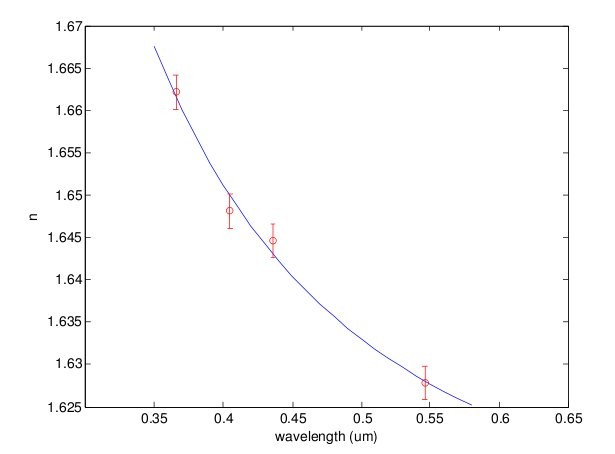
\includegraphics[width=0.9\linewidth]{figures/index_refraction.png}
    \caption{\small The measured index of refraction for flint glass. The curve shows the results of a fit to the form (say) of Eq. (\ref{eq:photoelectric_energy}).\cite{Kov_22}}
    \label{fig:index_refraction}
\end{figure}
\section{Conclusions}\label{sec:conclusion}

The final section of the paper should summarize your findings and emphasize what has been learned as a result of your work. Compare the new results with what was already known, and discuss research which could lead to an improved future understanding.

The context for this part of the paper should be firmly rooted in the discussion which appeared in the Theory section. There you have presented the case for obtaining a new and improved measurement of a physical constant, or testing the prediction of a physical theory. This is true even for work which is done as a student laboratory assignment!

Typically, a paper's concluding section does not emphasize the experimental aspects of the investigation, but rather how the measured results have advanced our state of knowledge. This is not to say that experimental issues are excluded from the Conclusions, just that they are not usually given an emphasis unless the project is primarily focused on a novel or significantly improved experimental method.
\section*{Appendix}

An appendix to a conventional journal article will typically contain either data in the form of one or more tables or figures, or additional explanatory text which may also include mathematical derivations. In our papers, only data tables and figures may be included, not text or mathematics.

When would you choose to put data in the Appendix, rather than in the Results section? Typically, data tables that appear as part of the Results are of limited length and complexity. The data we show in Table 1 are "not too long," and "not too complex." But if our data instead consisted of the mean terminal velocity of each of 10 oil drops in each of three electric field settings, then those results should appear in a table in the Appendix. Tables which appear in the Appendix should contain only a limited set of "distilled" data.

In some cases it may be useful to show one or more plots of the data, beyond those which appear in the Results. We may, for example, elect to include a figure showing "raw" data in the Appendix.

Each data table and figure in the Appendix must have a caption.

\bibliography{ref}
%%%%%%%%%%%%%%%%%%%%%%%%%%%%%%%%%%%%%%%%%%%%


\end{document}